%beamer

% Define a global usable date. Must come before StyleTut
%\newcommand{\mydate}{18.11.2016}

% Comment/uncomment this line to toggle handout mode
%\newcommand{\handout}{}

%% Beamer-Klasse im korrekten Modus
\ifdefined \handout
\documentclass[handout]{beamer} % Handout mode
\else
\documentclass{beamer}
\fi

%% UTF-8-Encoding
\usepackage[utf8]{inputenc}

% % \bigtimes abgeschrieben von http://tex.stackexchange.com/questions/14386/importing-a-single-symbol-from-a-different-font
% \DeclareFontFamily{U}{mathx}{\hyphenchar\font45}
% \DeclareFontShape{U}{mathx}{m}{n}{
%       <5> <6> <7> <8> <9> <10> gen * mathx
%       <10.95> mathx10 <12> <14.4> <17.28> <20.74> <24.88> mathx12
%       }{}
% \DeclareSymbolFont{mathx}{U}{mathx}{m}{n}
% \DeclareMathSymbol{\bigtimes}{\mathop}{mathx}{161}

\RequirePackage{xcolor}

\def\9{\square}
%\def\9{\blank}

% f"ur Aussagenlogik
\colorlet{alcolor}{blue}
\RequirePackage{tikz}
\usetikzlibrary{arrows.meta}
\newcommand{\alimpl}{\mathrel{\tikz[x={(0.1ex,0ex)},y={(0ex,0.1ex)},>={Classical TikZ Rightarrow[]}]{\draw[alcolor,->,line width=0.7pt,line cap=round] (0,0) -- (15,0);\path (0,-6);}}}
\newcommand{\aleqv}{\mathrel{\tikz[x={(0.1ex,0ex)},y={(0ex,0.1ex)},>={Classical TikZ Rightarrow[]}]{\draw[alcolor,<->,line width=0.7pt,line cap=round] (0,0) -- (18,0);\path (0,-6);}}}
\newcommand{\aland}{\mathbin{\raisebox{-0.6pt}{\rotatebox{90}{\texttt{\color{alcolor}\char62}}}}}
\newcommand{\alor}{\mathbin{\raisebox{-0.8pt}{\rotatebox{90}{\texttt{\color{alcolor}\char60}}}}}
%\newcommand{\ali}[1]{_{\mathtt{\color{alcolor}#1}}}
\newcommand{\alv}[1]{\mathtt{\color{alcolor}#1}}
\newcommand{\alnot}{\mathop{\tikz[x={(0.1ex,0ex)},y={(0ex,0.1ex)}]{\draw[alcolor,line width=0.7pt,line cap=round,line join=round] (0,0) -- (10,0) -- (10,-4);\path (0,-8) ;}}}
\newcommand{\alP}{\alv{P}} %ali{#1}}
%\newcommand{\alka}{\negthinspace\hbox{\texttt{\color{alcolor}(}}}
\newcommand{\alka}{\negthinspace\text{\texttt{\color{alcolor}(}}}
%\newcommand{\alkz}{\texttt{\color{alcolor})}}\negthinspace}
\newcommand{\alkz}{\text{\texttt{\color{alcolor})}}\negthinspace}
\newcommand{\AAL}{A_{AL}}
\newcommand{\LAL}{\hbox{\textit{For}}_{AL}}
\newcommand{\AxAL}{\hbox{\textit{Ax}}_{AL}}
\newcommand{\AxEq}{\hbox{\textit{Ax}}_{Eq}}
\newcommand{\AxPL}{\hbox{\textit{Ax}}_{PL}}
\newcommand{\AALV}{\hbox{\textit{Var}}_{AL}}
\newcommand{\MP}{\hbox{\textit{MP}}}
\newcommand{\GEN}{\hbox{\textit{GEN}}}
\newcommand{\W}{\ensuremath{\hbox{\textbf{w}}}\xspace}
\newcommand{\F}{\ensuremath{\hbox{\textbf{f}}}\xspace}
\newcommand{\WF}{\ensuremath{\{\W,\F\}}\xspace}
\newcommand{\val}{\hbox{\textit{val}}}
\newcommand{\valDIb}{\val_{D,I,\beta}}

\newcommand*{\from}{\colon}

% die nachfolgenden Sachen angepasst an cmtt
\newlength{\ttquantwd}
\setlength{\ttquantwd}{1ex}
\newlength{\ttquantht}
\setlength{\ttquantht}{6.75pt}
\def\plall{%
  \tikz[line width=0.67pt,line cap=round,line join=round,baseline=(B),alcolor] {
    \draw (-0.5\ttquantwd,\ttquantht) -- node[coordinate,pos=0.4] (lll){} (-0.25pt,-0.0pt) -- (0.25pt,-0.0pt) -- node[coordinate,pos=0.6] (rrr){} (0.5\ttquantwd,\ttquantht);
    \draw (lll) -- (rrr);
    \coordinate (B) at (0,-0.35pt);
  }%
}
\def\plexist{%
  \tikz[line width=0.67pt,line cap=round,line join=round,baseline=(B),alcolor] {
    \draw (-0.9\ttquantwd,\ttquantht) -- (0,\ttquantht) -- node[coordinate,pos=0.5] (mmm){} (0,0) --  (-0.9\ttquantwd,0);
    \draw (mmm) -- ++(-0.75\ttquantwd,0);
    \coordinate (B) at (0,-0.35pt);
  }\ensuremath{\,}%
}
\let\plexists=\plexist
\newcommand{\NT}[1]{\ensuremath{\langle\mathrm{#1} \rangle}}

\newcommand{\CPL}{\text{\itshape Const}_{PL}}
\newcommand{\FPL}{\text{\itshape Fun}_{PL}}
\newcommand{\RPL}{\text{\itshape Rel}_{PL}}
\newcommand{\VPL}{\text{\itshape Var}_{PL}}
\newcommand{\ATer}{A_{\text{\itshape Ter}}}
\newcommand{\ARel}{A_{\text{\itshape Rel}}}
\newcommand{\AFor}{A_{\text{\itshape For}}}
\newcommand{\LTer}{L_{\text{\itshape Ter}}}
\newcommand{\LRel}{L_{\text{\itshape Rel}}}
\newcommand{\LFor}{L_{\text{\itshape For}}}
\newcommand{\NTer}{N_{\text{\itshape Ter}}}
\newcommand{\NRel}{N_{\text{\itshape Rel}}}
\newcommand{\NFor}{N_{\text{\itshape For}}}
\newcommand{\PTer}{P_{\text{\itshape Ter}}}
\newcommand{\PRel}{P_{\text{\itshape Rel}}}
\newcommand{\PFor}{P_{\text{\itshape For}}}

\newcommand{\plka}{\alka}
\newcommand{\plkz}{\alkz}
%\newcommand{\plka}{\plfoo{(}}
%\newcommand{\plkz}{\plfoo{)}}
\newcommand{\plcomma}{\hbox{\texttt{\color{alcolor},}}}
\newcommand{\pleq}{{\color{alcolor}\,\dot=\,}}

% MODIFIED (DJ)
% previously: \newcommand{\plfoo}[1]{\mathtt{\color{alcolor}#1}}
\newcommand{\plfoo}[1]{\texttt{\color{alcolor}#1}}

\newcommand{\plc}{\plfoo{c}}
\newcommand{\pld}{\plfoo{d}}
\newcommand{\plf}{\plfoo{f}}
\newcommand{\plg}{\plfoo{g}}
\newcommand{\plh}{\plfoo{h}}
\newcommand{\plx}{\plfoo{x}}
\newcommand{\ply}{\plfoo{y}}
\newcommand{\plz}{\plfoo{z}}
\newcommand{\plR}{\plfoo{R}}
\newcommand{\plS}{\plfoo{S}}

\newcommand{\bv}{\mathrm{bv}}
\newcommand{\fv}{\mathrm{fv}}

%\newcommand{\AxAL}{\hbox{\textit{Ax}}_{AL}}
%\newcommand{\AALV}{\hbox{\textit{Var}}_{AL}}

%\renewcommand{\#}[1]{\literal{#1}}
\newcommand{\A}{\mathcal{A}}
\newcommand{\Adr}{\text{Adr}}
\newcommand{\ar}{\mathrm{ar}}
\newcommand{\ascii}[1]{\literal{\char#1}}
%\newcommand{\assert}[1]{\text{/\!\!/\ } #1}
\newcommand{\assert}[1]{\colorbox{black!7!white}{\ensuremath{\{\;#1\;\}}}}
\newcommand{\Assert}[1]{$\langle$\textit{#1}$\rangle$}
\newcommand{\B}{\mathcal{B}}
\newcommand{\bfmod}{\mathbin{\kw{ mod }}}
\newcommand{\bb}{{\text{bb}}}
\def\bottom{\hbox{\small$\pmb{\bot}$}}
\newcommand{\card}[1]{|#1|}
%\newcommand{\cod}{\mathop{\text{cod}}}  % ist in thwmathabbrevs
\newcommand{\Conf}{\mathcal{C}}
\newcommand{\define}[1]{\emph{#1}}
%\renewcommand{\dh}{d.\,h.\@\xspace}
%\newcommand{\Dh}{D.\,h.\@\xspace}
%\newcommand{\engl}[1]{engl.\xspace\emph{#1}}
\newcommand{\eps}{\varepsilon}
%\newcommand{\evtl}{evtl.\@\xspace}
\newcommand{\fbin}{\text{bin}}
\newcommand{\finv}{\text{inv}}
\newcommand{\fnum}{\text{num}}
\newcommand{\fNum}{{\text{Num}}}
\newcommand{\frepr}{\text{repr}}
\newcommand{\fRepr}{\text{Repr}}
\newcommand{\fZkpl}{\text{Zkpl}}
\newcommand{\fLen}{\text{Len}}
\newcommand{\fsem}{\text{sem}}
\providecommand{\fspace}{\mathord{\text{space}}}
\providecommand{\fSpace}{\mathord{\text{Space}}}
\providecommand{\ftime}{\mathord{\text{time}}}
\providecommand{\fTime}{\mathord{\text{Time}}}
\newcommand{\fTrans}{\text{Trans}}
\newcommand{\fVal}{\text{Val}}

% Modified (DJ)
\newcommand{\Val}{\text{Val}}

%\def\G{\mathbb{Z}}
\newcommand{\HT}[1]{\normalfont\textsc{HT-#1}}
\newcommand{\htr}[3]{\{#1\}\;#2\; \{#3\}}
\newcommand{\Id}{\text{I}}
%\newcommand{\ie}{i.\,e.\@\xspace}
\newcommand{\instr}[2]{\texttt{#1}\ \textit{#2}}
\newcommand{\Instr}[2]{\texttt{#1}\ \textrm{#2}}
\newcommand{\instrr}[3]{\texttt{#1}\ \textit{#2}\texttt{(#3)}}
\newcommand{\Instrr}[3]{\texttt{#1}\ \textrm{#2}\texttt{(#3)}}
\newcommand{\io}{\!\mid\!}
\usepackage{KITcolors}
\newcommand{\literal}[1]{\hbox{\textcolor{blue!95!white}{\textup{\texttt{\scalebox{1.11}{#1}}}}}}
%\newcommand{\literal}[1]{\hbox{\textcolor{KITblue!80!black}{\textup{\texttt{#1}}}}}
\def\kasten#1{\leavevmode\literal{\setlength{\fboxsep}{1pt}\fbox{\vrule  width 0pt height 1.5ex depth 0.5ex #1}}}
\newcommand{\kw}[1]{\ensuremath{\mathbf{#1}}}
\newcommand{\lang}[1]{\ensuremath{\langle#1\rangle}}
%\newcommand{\maw}{m.\,a.\,w.\@\xspace}
%\newcommand{\MaW}{M.\,a.\,w.\@\xspace}
\newcommand{\mdefine}[2][FOOBAR]{\define{#2}\def\foobar{FOOBAR}\def\optarg{#1}\ifx\foobar\optarg\def\optarg{#2}\fi\graffito{\optarg}}
\newcommand{\meins}{\rotatebox[origin=c]{180}{1}}
\newcommand{\Mem}{\text{Mem}}
\newcommand{\memread}{\text{memread}}
\newcommand{\memwrite}{\text{memwrite}}
\providecommand{\meta}[1]{\ensuremath{\langle}\textit{#1}\ensuremath{\rangle}}
%\newcommand{\N}{\mathbb{N}}
\newcommand{\NP}{\mathbf{NP}}
\newcommand{\Nadd}{N_{\text{add}}}
\newcommand{\Nmult}{N_{\text{mult}}}
\newcommand{\Oh}[1]{O\left(#1\right)}
\newcommand{\Om}[1]{\Omega\left(#1\right)}
\newcommand{\personname}[1]{\textsc{#1}}
\newcommand{\regname}[1]{\texttt{#1}}
\newcommand{\mima}{\textsc{Mima}\xspace}
\newcommand{\mimax}{\textsc{Mima-X}\xspace}

\def\Pclass{\text{\bfseries P}}
\def\PSPACE{\text{\bfseries PSPACE}}

\newcommand{\SPush}{\text{push}}
\newcommand{\SPop}{\text{pop}}
\newcommand{\SPeek}{\text{peek}}
\newcommand{\STop}{\text{top}}
\newcommand{\STos}{\text{\itshape tos}}
\newcommand{\SBos}{\text{\itshape bos}}

%\newcommand{\R}{\mathbb{R}}
\newcommand{\Rnullplus}{\R_0^{+}}
\newcommand{\Rplus}{\R_{+}}
\newcommand{\resp}{resp.\@\xspace}
\newcommand{\Sem}{\text{Sem}}
\newcommand{\sgn}{\mathop{\text{sgn}}}
\newcommand{\sqbox}{\mathop{\raisebox{-6.2pt}{\hbox{\hbox to 0pt{$^{^{\sqcap}}$\hss}$^{^{\sqcup}}$}}}}
\newcommand{\sqleq}{\sqsubseteq}
\newcommand{\sqgeq}{\sqsupseteq}
\newcommand{\Th}[1]{\Theta\left(#1\right)}
%\newcommand{\usw}{usw.\@\xspace}
\newcommand{\V}[1]{\hbox{\textit{#1}}}
\newcommand{\x}{\times}
\newcommand{\ZK}{\mathbb{K}}
%\newcommand{\Z}{\mathbb{Z}}
%\newcommand{\zB}{z.\,B.\@\xspace}
%\newcommand{\ZB}{Z.\,B.\@\xspace}
% \newcommand{\bb}{{\text{bb}}}
% \def\##1{\hbox{\textcolor{darkblue}{\texttt{#1}}}}
% \def\A{\mathcal{A}}
% \newcommand{\0}{\#0}
% \newcommand{\1}{\#1}
% \newcommand{\Obj}{\text{Obj}}
% \newcommand{\start}{\mathop{\text{start}}}
% \newcommand{\compactlist}{\addtolength{\itemsep}{-\parskip}}
% \newcommand{\fval}{\text{val}}
% \newcommand{\lang}[1]{\ensuremath{\langle#1\rangle}}
% \newcommand{\io}{\!\mid\!}
% \def\sqbox{\mathop{\raisebox{-6.2pt}{\hbox{\hbox to 0pt{$^{^{\sqcap}}$\hss}$^{^{\sqcup}}$}}}}
% \def\sqleq{\sqsubseteq}
% \def\sqgeq{\sqsupseteq}
\def\Td{T_{\overline{d}}}
% \newcommand{\csym}[1]{\ensuremath{\#{c}_{\#{\hbox{\scriptsize #1}}}}}
% \newcommand{\F}{\ensuremath{\mathcal{F}}}
% \newcommand{\fsym}[2]{\ensuremath{\#{f}^{\#{\hbox{\scriptsize #1}}}_{\#{\hbox{\scriptsize #2}}}}}
% \newcommand{\rsym}[2]{\ensuremath{\#{R}^{\#{\hbox{\scriptsize #1}}}_{\#{\hbox{\scriptsize #2}}}}}
% \newcommand{\xsym}[1]{\ensuremath{\#{x}_{\#{\hbox{\scriptsize #1}}}}}
% \newcommand{\I}{\mathcal{I}}
% ********************************************************************

\usepackage{../TutTexbib/thwregex}
\usepackage{environ}
\usepackage{bm}
\usepackage{calc}
\usepackage{varwidth}
\usepackage{wasysym}
\usepackage{mathtools}

%% Tabellen
\usepackage{array}
\usepackage{multicol}

%% Bibliotheken für viele mathematische Symbole
\usepackage{amsmath, amsfonts, amssymb}



% This is a configuration file with personal tutor information.
% It is therefore excluded from the git repository, so changes in this file will not conflict in git commits.

% Copy this template, rename to config.tex and add your information below.

\newcommand{\myname}{Lukas Morawietz}
\newcommand{\mymail}{lukas.morawietz@gmail.com} % Consider using your named student mail address to keep your u**** account private.
\newcommand{\mytutnumber}{31}

% Don't forget to update ILIAS url. WARNING: Underscores '_' and Ampersands '&' have to be escaped with backslashes '\'. Blame TeX, not me.
\newcommand{\myILIASurl}{https://ilias.studium.kit.edu/ilias.php?ref\_id=855240\&cmdClass=ilrepositorygui\&cmdNode=5r\&baseClass=ilrepositorygui}

% Uncommenting this will print Socrative info with here defined roomname whenever \Socrative is called.
% (Otherwise, \Socrative will remain silent.)
% \newcommand{\mysocrativeroom}{???}

%\def\ThassesTut{}
\def\DanielsTut{}

\newcommand{\aboutMeFrame}{
	\begin{frame}{Über mich}
		\myname \\
		Informatik, 9. Fachsemester (Bachelor)
		% Lebensgeschichte...
		% Stammbaum...
		% Aufarbeitung der eigenen Todesser-Vergangenheit...
	\end{frame}
}

\def\thisyear{2019}

% Update date of exam
\def\myKlausurtermin{18.~März~2020, 14:00–16:00~Uhr}

\def\mydate#1{
		  \ifnum#1=1\relax	  23. Oktober \thisyear \
	\else \ifnum#1=2\relax	  30. Oktober \thisyear \
	\else \ifnum#1=3\relax    06. November \thisyear \
	\else \ifnum#1=4\relax    13. November \thisyear \
	\else \ifnum#1=5\relax    20. November \thisyear \
	\else \ifnum#1=6\relax    27. November \thisyear \
	\else \ifnum#1=7\relax    04. Dezember \thisyear \
	\else \ifnum#1=8\relax    11. Dezember \thisyear \
	\else \ifnum#1=9\relax    18. Dezember \thisyear \
	\else \ifnum#1=10\relax   08. Januar \nextyear \
	\else \ifnum#1=11\relax   15. Januar \nextyear \
	\else \ifnum#1=12\relax   22. Januar \nextyear \
	\else \ifnum#1=13\relax   29. Januar \nextyear \
	\else \ifnum#1=14\relax   05. Februar \nextyear \
	\else \textbf{Datum undefiniert!} 
	\fi\fi\fi\fi\fi\fi\fi\fi\fi\fi\fi\fi\fi\fi
}

\def\mylasttimestext{Was letztes Mal geschah...}

\colorlet{beamerlightred}{red!40}
\colorlet{beamerlightgreen}{green!50}
\colorlet{beamerlightyellow}{yellow!50}
\colorlet{lightred}{red!30}
\colorlet{lightgreen}{green!40}
\colorlet{lightyellow}{yellow!50}
\colorlet{fullred}{red!60}
\colorlet{fullgreen}{green}

\definecolor{myalertcolor}{rgb}{1,0.33,0.24}
\setbeamercolor{alerted text}{fg=myalertcolor}

% Flag to toggle display of KIT Logo.
% If you want to conform to the official logo guidelines, 
% you are not allowed to use the logo and should disable it
% using the following flag. Just saying.
% (But it's too beautiful, so best leave this commented. :P)
%\newcommand{\noKITLogo}{}

% Toggle handout mode by including the following line before including PraeambelTut
% and removing the % at the start (but do NOT remove the % char here, otherwise handout mode will always be on!)
% Please keep handout mode off in all commits!

% \newcommand{\handout}{}



% define custom \handout command flag if handout mode is toggled  #DirtyAsHellButWell...
\only<beamer:0>{\def\handout{}} %beamer:0 == handout mode

\newcommand{\R}{\mathbb{R}}
\newcommand{\N}{\mathbb{N}}
\newcommand{\Z}{\mathbb{Z}}
\newcommand{\Q}{\mathbb{Q}}
\newcommand{\BB}{\mathbb{B}}
\newcommand{\C}{\mathbb{C}}
\newcommand{\K}{\mathbb{K}}
\newcommand{\G}{\mathbb{G}}
\newcommand{\nullel}{\mathcal{O}}
\newcommand{\einsel}{\mathds{1}}
\newcommand{\Pot}{\mathcal{P}}
\renewcommand{\O}{\text{O}}

\def\word#1{\hbox{\textcolor{blue}{\texttt{#1}}}}
\let\literal\word
\def\mword#1{\hbox{\textcolor{blue}{$\mathtt{#1}$}}}  % math word
\def\sp{\scalebox{1}[.5]{\textvisiblespace}}
\def\wordsp{\word{\sp}}

%\newcommand{\literal}[1]{\textcolor{blue}{\texttt{#1}}}
\newcommand{\realTilde}{\textasciitilde \ }
\newcommand{\setsize}[1]{\ensuremath{\left\lvert #1 \right\rvert}}
\let\size\setsize
\newcommand{\set}[1]{\left\{#1\right\}}
\newcommand{\tuple}[1]{\left(#1\right)}
\newcommand{\normalvar}[1]{\text{$#1$}}

% Modified by DJ
\let\oldemptyset\emptyset
\let\emptyset\varnothing % proper emptyset

%\definecolor{myRed}{RGB}{255,75,20}
%\colorlet{myGreen}{KITpalegreen}

%\newcounter{tfqtempcount}
%\newcommand{\truefalseQ}[4]{
%	\setcounter{tfqtempcount}{#1}
%	\addtocounter{tfqtempcount}{1}
%	\truefalseQuestion{#1}{\value{tfqtempcount}}{#2}{#3}{#4}
%}

%\newcommand{\truefalseQuestion}[5]{\item<#1-|handout:#1-> \color<#2-|handout:#2->{#3} #4 \qquad \visible<#2-|handout:#2->{#5}}

\newcommand{\boder}{\ensuremath{\mathbin{\textcolor{blue}{\vee}}}\xspace}
\newcommand{\bund}{\ensuremath{\mathbin{\textcolor{blue}{\wedge}}}\xspace}
\newcommand{\bimp}{\ensuremath{\mathrel{\textcolor{blue}{\to}}}\xspace}
\newcommand{\bgdw}{\ensuremath{\mathrel{\textcolor{blue}{\leftrightarrow}}}\xspace}
\newcommand{\bnot}{\ensuremath{\textcolor{blue}{\neg}}\xspace}
\newcommand{\bone}{\ensuremath{\textcolor{blue}{1}}\text{}}
\newcommand{\bzero}{\ensuremath{\textcolor{blue}{0}}\text{}}
\newcommand{\bleftBr}{\ensuremath{\textcolor{blue}{\texttt{(}}}\text{}}
\newcommand{\brightBr}{\ensuremath{\textcolor{blue}{\texttt{)}}}\text{}}

\newcommand{\plB}{\plfoo{B}}
\newcommand{\plE}{\plfoo{E}}

\newcommand{\summe}[2]{\sum\limits_{#1}^{#2}}
\newcommand{\limes}[1]{\lim\limits_{#1}}

%\newcommand{\numpp}{\advance \value{weeknum} by -2 \theweeknum \advance \value{weeknum} by 2}
%\newcommand{\nump}{\advance \value{weeknum} by -1 \theweeknum \advance \value{weeknum} by 1}

\newcommand{\mycomment}[1]{}
\newcommand{\Comment}[1]{}

%% DISCLAIMER START 
% It is INSANELY IMPORTANT NOT TO DO THIS OUTSIDE BEAMER CLASS! IN ARTCILE DOCUMENTS, THIS IS VERY LIKELY TO BUG AROUND!
\makeatletter%
\@ifclassloaded{beamer}%
{
	% TODO 
	% no time...
	% redefine section to ignore multiple \section calls with the same title
}%
{
	\errmessage{ERROR: section command redefinition outside of beamer class document! Please contact the author of this code.}
}%
\makeatother%
%% DISCLAIMER END

\newcounter{abc}
\newenvironment{alist}{
  \begin{list}{(\alph{abc})}{
      \usecounter{abc}\setlength{\leftmargin}{8mm}\setlength{\labelsep}{2mm}
    }
}{\end{list}}


\newcommand{\stdarraystretch}{1.20}
\renewcommand{\arraystretch}{\stdarraystretch}  % for proper row spacing in tables

\newcommand{\morescalingdelimiters}{   % for proper \left( \right) typography
	\delimitershortfall=-1pt  
	\delimiterfactor=1
}

\newcommand{\centered}[1]{\vspace{-\baselineskip}\begin{center}#1\end{center}\vspace{-\baselineskip}}

% for \implitem and \item[bla] stuff to look right:
\setbeamercolor*{itemize item}{fg=black}
\setbeamercolor*{itemize subitem}{fg=black}
\setbeamercolor*{itemize subsubitem}{fg=black}

\setbeamercolor*{description item}{fg=black}
\setbeamercolor*{description subitem}{fg=black}
\setbeamercolor*{description subsubitem}{fg=black}

\renewcommand{\qedsymbol}{\textcolor{black}{\openbox}}

\renewcommand{\mod}{\mathop{\textbf{mod}}}
\renewcommand{\div}{\mathop{\textbf{div}}}

\newcommand{\ceil}[1]{\left\lceil#1\right\rceil}
\newcommand{\floor}[1]{\left\lfloor#1\right\rfloor}
\newcommand{\abs}[1]{\left\lvert #1 \right\rvert}
\newcommand{\Matrix}[1]{\begin{pmatrix} #1 \end{pmatrix}}
\newcommand{\braced}[1]{\left\lbrace #1 \right\rbrace}

\def\fract#1/#2 {\frac{#1}{#2}} % ! Trailing space is crucial!
\def\dfract#1/#2 {\dfrac{#1}{#2}} % ! Trailing space is crucial!

\newcommand{\Mid}{\;\middle|\;}

\let\after\circ

\def\·{\cdot}
\def\*{\cdot}
\def\?>{\ensuremath{\rightsquigarrow}}  % Fuck you, Latex

\newcommand{\tight}[1]{{\renewcommand{\arraystretch}{0.76} #1}}
\newcommand{\stackedtight}[1]{{\renewcommand{\arraystretch}{0.76} \begin{matrix} #1 \end{matrix}} }
\newcommand{\stacked}[1]{\begin{matrix} #1 \end{matrix} }
\newcommand{\casesl}[1]{\delimitershortfall=0pt  \left\lbrace\hspace{-.3\baselineskip}\begin{array}{ll} #1 \end{array}\right.}
\newcommand{\casesr}[1]{\delimitershortfall=0pt  \left.\begin{array}{ll} #1 \end{array}\hspace{-.3\baselineskip}\right\rbrace}
\newcommand{\caseslr}[1]{\delimitershortfall=0pt  \left\lbrace\hspace{-.3\baselineskip}\begin{array}{ll} #1 \end{array}\hspace{-.3\baselineskip}\right\rbrace}

\def\q#1uad{\ifnum#1=0\relax\else\quad\q{\the\numexpr#1-1\relax}uad\fi}
% e.g. \q1uad = \quad, \q2uad = \qquad etc.

\newcommand{\qqquad}{\q3uad}

\newcommand{\impl}{\ifmmode\ensuremath{\mskip\thinmuskip\Rightarrow\mskip\thinmuskip}\else$\Rightarrow$\fi\xspace}
\newcommand{\Impl}{\ifmmode\implies\else$\Longrightarrow$\fi\xspace}

\newcommand{\derives}{\Rightarrow}

\newcommand{\gdw}{\ifmmode\mskip\thickmuskip\Leftrightarrow\mskip\thickmuskip\else$\Leftrightarrow$\fi\xspace}
\newcommand{\Gdw}{\ifmmode\iff\else$\Longleftrightarrow$\fi\xspace}

\newcommand{\symbitemnegoffset}{\hspace{-.5\baselineskip}}
\newcommand{\implitem}{\item[\impl\symbitemnegoffset]}
\newcommand{\Implitem}{\item[\Impl\symbitemnegoffset]}


\newcommand{\forcenewline}{\mbox{}\\}


% proper math typography
\newcommand{\functionto}{\longrightarrow}
\renewcommand{\geq}{\geqslant}
\renewcommand{\leq}{\leqslant}
\let\oldsubset\subset
\renewcommand{\subset}{\subseteq} % for all idiots out there using subset

\newenvironment{threealign}{%
	\[
	\begin{array}{r@{\ }c@{\ }l}
}{%
	\end{array}	
	\]
}

\newcommand{\concludes}{ \\ \hline  }
\newcommand{\deduction}[1]{
	\begin{varwidth}{.8\linewidth}
		\begin{tabular}{>{$}c<{$}}
			#1
		\end{tabular}
	\end{varwidth}	
}

\definecolor{hoareorange}{rgb}{1,.85,.6}
\newcommand{\hoareassert}[1]{\setlength{\fboxsep}{1pt}\setlength{\fboxrule}{-1.4pt}\fcolorbox{white}{hoareorange}{\ensuremath{\{\;#1\;\}}}\setlength\fboxrule{\defaultfboxrule}\setlength{\fboxsep}{3pt}}

\newcommand{\mailto}[1]{\href{mailto:#1}{{\textcolor{blue}{\underline{#1}}}}}
\newcommand{\urlnamed}[2]{\href{#2}{\textcolor{blue}{\underline{#1}}}}
\renewcommand{\url}[1]{\urlnamed{#1}{#1}}

\newcommand{\hanging}{\hangindent=0.7cm}
\newcommand{\indented}{\hanging}

%requires \thisyear to be defined (s. config.tex)!
\edef\nextyear{\the\numexpr\thisyear+1\relax}


% --- \frameheight constant ---
\newlength\fullframeheight
\newlength\framewithtitleheight
\setlength\fullframeheight{.92\textheight}
\setlength\framewithtitleheight{.86\textheight}

\newlength\frameheight
\setlength\frameheight{\fullframeheight}

\let\frametitleentry\relax
\let\oldframetitle\frametitle
\def\newframetitle#1{\global\def\frametitleentry{#1}\if\relax\frametitleentry\relax\else\setlength\frameheight{\framewithtitleheight}\fi\oldframetitle{#1}}
\let\frametitle\newframetitle

\def\newframetitleoff{\let\frametitle\oldframetitle}
\def\newframetitleon{\let\frametitle\newframetitle}
% --- \frameheight constant end ---



\newenvironment{headframe}{\Huge THIS IS AN ERROR. PLEASE CONTACT THE ADMIN OF THIS TEX CODE. (headframe env def failed)}{}
\RenewEnviron{headframe}[1][]{
	\begin{frame}\frametitle{\ }
		\centering
		\Huge\textbf{\textsc{\BODY} \\
		}
		\Large {#1}
		\frametitle{\ }
	\end{frame}
}


\makeatletter
% Provides color if undefined.
\newcommand{\colorprovide}[2]{%
	\@ifundefinedcolor{#1}{\colorlet{#1}{#2}}{}}
\makeatother


\colorprovide{lightred}{red!30}
\colorprovide{lightgreen}{green!40}
\colorprovide{lightyellow}{yellow!50}
\colorprovide{beamerlightred}{lightred}
\colorprovide{beamerlightgreen}{lightgreen}
\colorprovide{beamerlightyellow}{lightyellow}
\colorprovide{fullred}{red!60}
\colorprovide{fullgreen}{green}
\definecolor{darkred}{RGB}{115,48,38}
\definecolor{darkgreen}{RGB}{48,115,38}
\definecolor{darkyellow}{RGB}{100,100,0}

\only<handout:0>{\colorlet{adaptinglightred}{beamerlightred}}
\only<handout:0>{\colorlet{adaptinglightgreen}{beamerlightgreen}}
\only<handout:0>{\colorlet{adaptinglightred}{beamerlightred}}
\only<beamer:0>{\colorlet{adaptinglightred}{lightred}}
\only<beamer:0>{\colorlet{adaptinglightgreen}{lightgreen}}
\only<beamer:0>{\colorlet{adaptinglightred}{lightred}}
\only<handout:0>{\colorlet{adaptingred}{lightred}}
\only<beamer:0>{\colorlet{adaptingred}{fullred}}
\only<handout:0>{\colorlet{adaptinggreen}{lightgreen}}
\only<beamer:0>{\colorlet{adaptinggreen}{fullgreen}}



\newcommand{\TrueQuestion}[1]{
	\TrueQuestionE{#1}{}
}

\newcommand{\YesQuestion}[1]{
	\YesQuestionE{#1}{}
}

\newcommand{\FalseQuestion}[1]{
	\FalseQuestionE{#1}{}
}

\newcommand{\NoQuestion}[1]{
	\NoQuestionE{#1}{}
}

\newcommand{\DependsQuestion}[1]{
	\DependsQuestionE{#1}{}
}

\newcommand{\QuestionVspace}{\vspace{4pt}}
\newcommand{\QuestionParbox}[1]{\begin{varwidth}{.85\linewidth}#1\end{varwidth}}
\newcommand{\ExplanationParbox}[1]{\begin{varwidth}{.97\linewidth}#1\end{varwidth}}
\colorlet{questionlightgray}{gray!23}
\let\defaultfboxrule\fboxrule

% #1: bg color
% #2: fg color short answer
% #3: short answer text
% #4: question
% #5: explanation
\newcommand{\GenericQuestion}[5]{
	\setlength\fboxrule{2pt}
	\only<+|handout:0>{\hspace{-2pt}\fcolorbox{white}{questionlightgray}{\QuestionParbox{#4} \quad\textbf{?}}}
	\visible<+->{\hspace{-2pt}\fcolorbox{white}{#1}{\QuestionParbox{#4} \quad\textbf{\textcolor{#2}{#3}}} \ExplanationParbox{#5}} \\
	\setlength\fboxrule{\defaultfboxrule}
}

% #1: Q text
% #2: Explanation
\newcommand{\TrueQuestionE}[2]{
	\GenericQuestion{adaptinglightgreen}{darkgreen}{Wahr.}{#1}{#2}
}

% #1: Q text
% #2: Explanation
\newcommand{\YesQuestionE}[2]{
	\GenericQuestion{adaptinglightgreen}{darkgreen}{Ja.}{#1}{#2}
}

% #1: Q text
% #2: Explanation
\newcommand{\FalseQuestionE}[2]{
	\GenericQuestion{adaptinglightred}{darkred}{Falsch.}{#1}{#2}
}

% #1: Q text
% #2: Explanation
\newcommand{\NoQuestionE}[2]{
	\GenericQuestion{adaptinglightred}{darkred}{Nein.}{#1}{#2}
}

% #1: Q text
% #2: Explanation
\newcommand{\DependsQuestionE}[2]{
	\GenericQuestion{adaptinglightyellow}{darkyellow}{Je nachdem!}{#1}{#2}
}

\ifnum\thisyear=2017 \else \errmessage{Old ILIAS link inside preamble. Please update.} \fi

\newcommand{\ILIAS}{\urlnamed{ILIAS}{https://ilias.studium.kit.edu/ilias.php?ref\_id=729057\&cmdClass=ilrepositorygui\&cmdNode=75\&baseClass=ilrepositorygui}\xspace}

\newcommand{\Socrative}{\only<handout:0>{socrative.com $\qquad \?> $ Student login \\ Raumname:  \mysocrativeroom\\ \medskip}}

\newcommand{\thasse}[1]{
	\ifdefined\ThassesTut #1\xspace \else\fi
}
\newcommand{\daniel}[1]{
	\ifdefined\DanielsTut #1\xspace \else\fi
}
\newcommand{\thassedaniel}[2]{\ifdefined\ThassesTut #1\else\ifdefined\DanielsTut #2\fi\fi\xspace}

\ifdefined\ThassesTut \ifdefined\DanielsTut \errmessage{ERROR: Both ThassesTut and DanielsTut flags are set. This is most likely an error. Please check your config.tex file.} \else \fi \else \ifdefined\DanielsTut \else \errmessage{ERROR: Neither ThassesTut  nor DanielsTut flags are set. This is most likely an error. Please check your config.tex file.} \fi\fi

%\newcommand{\sgn}{\text{sgn}}


% Das ist der KIT-Stil
%\usepackage{../TutTexbib/beamerthemekit}
\usepackage[deutsch,titlepage0]{../TutTexbib/KIT/beamerthemeKITmod}
\TitleImage[width=\titleimagewd]{../figures/titlepage.jpg}
%\usetheme[deutsch,titlepage0]{KIT}

% Include PDFs
\usepackage{pdfpages}

% Libertine font (Original GBI font)
\usepackage{libertine}
%\renewcommand*\familydefault{\sfdefault}  %% Only if the base font of the document is to be sans serif

% Nicer math symbols
\usepackage{eulervm}
%\usepackage{mathpazo}
\renewcommand\ttdefault{cmtt} % Computer Modern typewriter font, see lecture slides.

%% Deutsche Silbentrennung und Beschriftungen
\usepackage[ngerman]{babel}



\usepackage{csquotes}



%% Anzeigetiefe für Inhaltsverzeichnis: 1 Stufe
\setcounter{tocdepth}{1}

%% Schönere Schriften
\usepackage[TS1,T1]{fontenc}

%% Bibliothek für Graphiken
\usepackage{graphicx}

%% der wird sowieso in jeder Datei gesetzt
%%\graphicspath{{../figures/}}

%% Hyperlinks
\usepackage{hyperref}
% I don't know why, but this works and only includes sections and NOT subsections in the pdf-bookmarks.
\hypersetup{bookmarksdepth=subsection} 

%\usepackage{lmodern}
\usepackage{colortbl}
\usepackage[absolute,overlay]{textpos}
\usepackage{listings}
\usepackage{forloop}
%\usepackage{algorithmic} % PseudoCode package 

\usepackage{tikz}
\usetikzlibrary{matrix}
\usetikzlibrary{arrows.meta}
\usetikzlibrary{automata}
\usetikzlibrary{tikzmark}

% Needed for gbi-macros
\usepackage{xspace}

%%%%%%%%%%%% INHALT %%%%%%%%%%%%%%%%

%% Wochennummer
\newcounter{weeknum}



%% Titelinformationen
\title[GBI-Tutorium \mytutnumber, Woche \theweeknum]{Grundbegriffe der Informatik \\ Tutorium \mytutnumber}

\subtitle{Woche \theweeknum \ | \mydate{\theweeknum} \\ \myname \ \  \normalfont (\mailto{\mymail})}
\author[\myname]{\myname}
\institute{KIT -- Karlsruher Institut für Technologie}
\date{\mydate{\theweeknum}\ }

% Modified, DJ (better safe than sorry)
\AuthorTitleSep{ – }

%% Titel einfügen
\newcommand{\titleframe}{\frame{\titlepage}}

%% Alles starten mit \starttut{X}
\newcommand{\starttut}[1]{\setcounter{weeknum}{#1}\titleframe\frame{\frametitle{Inhalt}\tableofcontents} \AtBeginSection[]{%
\begin{frame}
	\tableofcontents[currentsection]
\end{frame}\addtocounter{framenumber}{-1}}}


\newcommand{\framePrevEpisode}{
	\begin{headframe}
		\mylasttimestext
	\end{headframe}
}

%% Legacy: Lastframe. Not for further usage!
\newcommand{\lastframetitled}[5]{
	\frame[plain]{
		\vspace{-#2pt}
		\begin{figure}[H]
			\centering
			\LARGE \textbf{\textsc{#5}} \\
			\vspace{.2\baselineskip}
			\includegraphics[scale=#1]{#3}
			\vspace{-7pt}
			\caption{ \texttt{\url{#4}} }
		\end{figure} 
	}
}
\newcommand{\lastframe}[4]{\xkcdframe{#1}{#2}{#3}{#4}{}}
\newcommand{\xkcdframe}[5]{
	\frame[plain]{
		\vspace{-#2pt}
		\begin{figure}[H]
			\centering
			\includegraphics[scale=#1]{#3}
			\vspace{-7pt}
			\caption{ \texttt{\url{#4}} }
			\vspace{5pt}
			#5
		\end{figure} 
	}
}

%% Wörter
\newcommand{\code}[1]{$\mathbf{#1}$}

%% Sterne

\newcounter{starsc}
\newcommand{\stars}[1]{
	\hfill
	\begin{minipage}{100px}
		\forloop{starsc}{0}{\value{starsc} < #1}%
		{%
			
\includegraphics[scale=0.05]{star-full.pdf} \hspace*{1px}
		}%
		\forloop{starsc}{\value{starsc}}{\value{starsc} < 5}%
		{%
			
\includegraphics[scale=0.05]{star-empty.pdf} \hspace*{1px}
		}
		\vspace*{2px}
	\end{minipage}
}

% No stars for me...
\renewcommand{\stars}[1]{}

\newcommand{\slideThanks}{
	\begin{frame}
		\frametitle{Credits}
		\begin{block}{}
			Vorgänger dieses Foliensatzes wurden erstellt von:\\[1em]
			Thassilo Helmold \\
			Philipp Basler \\
			Nils Braun \\
			Dominik Doerner \\
			Ou Yue \\
		\end{block}
	\end{frame}
}

%% Verbatim
\usepackage{moreverb}

\graphicspath{{../figures/}}

\morescalingdelimiters

\begin{document}
\starttut{4}

\begin{frame}{Übungsblätter}
	
	Schnitt: \thassedaniel{XXX}{XXX} / 23~Punkte
	
	\begin{itemize}
		\item Erstmal: Volle Punktzahl ist utopisch. Fehler macht man, um draus zu lernen – dazu sind ÜBs da
		\item Versucht alle Aufgaben zu bearbeiten (sofern es Sinn macht)
		\item Wenn keine Begründung/Beweis gefordert ist, müsst ihr keinen angeben.
		\item Nicht mehrere Alternativen angeben, unter denen ich mir die richtige heraussuchen soll. (That's \emph{your} job!)
		\item \textbf{TACKERN} und \textbf{DECKBLÄTTER}! Sonst \alert{\textbf{null Punkte}}!
		\item Bitte die Aufgabenblätter nicht komplett mitabgeben (Deckblatt reicht), sonst wird mein Stapel so fett. \smiley
	\end{itemize}
	
\end{frame}

\begin{frame}[t]{Übungsblätter: Häufige Fehler}
	
		\TrueQuestionE{Beweise fängt man mit der Behauptung an.}{}
		\FalseQuestionE{Wenn wir $A$ schreiben, ist das immer eine Menge.}{Das muss man \textbf{explizit} angeben.}
		\FalseQuestionE{Ein Beispiel langt als Beweis.}{...bis ein anderes Beispiel herkommt, bei dem es kaputt geht... \\
			\impl eine Behauptung \textbf{widerlegen} geht mit nem Beispiel sehr gut!}
			%Mit einem Beispiel kann man eine Behauptung widerlegen, es zeigt aber nicht die Allgemeingültigkeit}
		% Modified by DJ (a more subtle version):
		\FalseQuestionE{$\setsize{M} = M$ für $M \subseteq \N$.}{$\setsize{M}$ ist die \textbf{Anzahl} der Elemente in $M$. Nix mit „Betrag“.}
	
	\medskip

	%TODO
	\pause[9]
	Wenn ihr eine Formel aufstellt, dann \textbf{prüft das Ergebnis für kleine Werte}.\\[0.2em]
	90~\% der falschen Antworten in 1.6.c) haben schon für $n \in \{0, 1\}$ nicht gestimmt.\\[0.5em]
	
	%TODO
	\pause[10]
	Passt auf, was eure Variablen sind und welche Operationen ihr darauf anwenden könnt. Mengen kann man nicht mit $\bund$ und $\boder$ verknüpfen
\end{frame}

\framePrevEpisode

\begin{frame}{Rückblick}
	\begin{itemize}
		\item \textbf{Aussagen} sind Sätze, die wahr oder falsch sind
		\item Wir können Aussagen mit \textbf{Konnektiven} zusammenbauen: \\
		\bund, \boder, \bnot, \bimp
		\item \textbf{Aussagevariablen} helfen dabei, konkrete Inhalte zu ignorieren 
		\item \textbf{Interpretationen} liefern Wahrheitswerte zu Variablen
		\item $val_I(\·)$ liefert Wahrheitswert für ganze Formel (rekursiv)
	\end{itemize}
\end{frame}


\section{Aussagenlogik}

\begin{frame}{Modelle}
	\begin{Definition}
		Sei $G$ eine aussagenlogische Formel. \\
		Eine Interpretation $I$ heißt \textbf{Modell} von $G$, wenn gilt: \quad $val_I(G) = \W$. \\
		\pause
		\medskip
		Sei $\Gamma$ eine Formelmenge.
		Eine Interpretation $I$ heißt \textbf{Modell} von $\Gamma$, wenn für alle Formeln $G \in  \Gamma$ gilt: \quad $val_I(G) = \W$.
	\end{Definition}
	\bigskip
	\pause
	\begin{block}{Schreibweisen}
		$\Gamma \models G$: jedes Modell von $\Gamma$ auch Modell von $G$ \\
		Beispiel: \quad $\set{A,B,C} \models G$ \quad Jedes Modell von $A, B$ \textbf{und} $C$ ist auch Modell von $G$ \\
		\medskip
		Schreibe $H \models G$ statt $\set{H} \models G$ \\
		\medskip
		Schreibe $\models G$ statt $\set{} \models G$ \\
		\impl G ist \emph{Tautologie} oder \emph{allgemeingültig} 
	\end{block}
\end{frame}

\begin{frame}{Modelle}
	\begin{Definition}
		Eine Formel $G$ heißt \textbf{erfüllbar}, wenn für mindestens ein $I$ wahr. \\
		
	\end{Definition}
	\pause
	\begin{Beispiel}
		Alle Modelle von \mword{(C \boder \bnot C) \bimp \left(\bnot(B \bimp A)\right)}? \\
		\pause
		\impl $I_1, I_2 \from \set{\word A, \word B, \word C} \functionto \BB, \; 
		I_1(v) = 
		\caseslr{\F, & v = \word A \\
				\W, & v = \word B \\
				\W, & v = \word C}, \;
		I_2(v) = 
		\caseslr{\F, & v = \word A \\
				\W, & v = \word B \\
				\F, & v = \word C}$. \\
		\impl Formel \emph{erfüllbar}. \\
		\pause
		\medskip
		Alle Modelle von \mword{\bnot(C \bimp C)}? \\
		\pause
		\impl Gibt keine, Formel \emph{unerfüllbar}.
	\end{Beispiel}
\end{frame}

\begin{frame}{Tautologie, Äquivalenz}
	\begin{Definition}
		Eine Formel $G$ heißt \textbf{Tautologie}, wenn für alle möglichen $I$ wahr. \\
		\pause
		\medskip
		Kurzschreibweise: Für Formeln $G$ und $H$ ist \\
		$$\bleftBr G \bgdw H \brightBr :\equiv \bleftBr\bleftBr G \bimp H \brightBr \bund \bleftBr H \bimp G\brightBr\brightBr$$ \\
		\medskip
		\alert{\textbf{Bitte aufpassen mit Pfeilen: \quad $\bgdw$ vs. $\gdw$ \quad $\bimp$ vs. $\impl$}}
	\end{Definition}
	\pause
	\begin{block}{Lemma}
		Für Formeln $G$ und $H$ gilt \\
		\[ G \equiv H \quad \text{ genau dann, wenn } \quad G \bgdw H \text{ Tautologie ist.} \]
	\end{block}
	\pause
	\begin{Beispiel}
		\centered{$\bnot\bnot G \bgdw G$ ist Tautologie, also $\bnot\bnot G \equiv G$}
	\end{Beispiel}
\end{frame}

\begin{frame}{Aussagenkalkül}
	\begin{block}{Was ist ein Kalkül?}
		\begin{itemize}
			\item Ein \emph{Rechensystem}: \; \textbf{Dinge} und was man mit ihnen \textbf{anstellen} darf. \\
			Bsp.: \quad $\R$ und $+, -, \·, /$ \qquad Schachbrett, Figuren und Zugregeln
		\end{itemize}
	\end{block}
	\pause
	\begin{block}{Aussagenkalkül}
		Haben
		\begin{itemize}
			\item Syntaktisch korrekte Formeln $For_{AL}$ \\
			\impl können erfüllbar sein oder nicht 
			\item Davon nennen wir einige bestimmte \textbf{Axiome} \\
			\impl setzen wir als Tautologien voraus
			\item Eine \emph{Schlussregel}: \textbf{Modus Ponens} \\
			...um neue Tautologien zu konstruieren
		\end{itemize}
	\end{block}
\end{frame}

\begin{frame}{Axiome, Modus Ponens}
	\begin{block}{Axiome}
		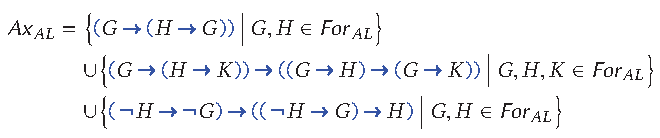
\includegraphics[width=.90\linewidth]{../figures/Axiome} \\
		Wir bestimmen: Das sind unsere „Basis-Tautologien“.
	\end{block}
	\pause
	\begin{block}{Modus Ponens (MP)}
		
		\begin{columns}[T] 
			\begin{column}[T]{.45\textwidth} 
				\vspace{-.6\baselineskip}
				\begin{itemize}
					\item<2-> Wenn $G$ gilt
					\item<2-> und $G \bimp H$ gilt \\ \mbox{}
					\implitem<2-> dann gilt auch $H$.
					\item<4-> Schreibweise: \deduction{G \qquad G \bimp H \concludes H} 
				\end{itemize}
			\end{column}
			\hspace{-2\baselineskip}
			\begin{column}[T]{.55\textwidth} 
				\vspace{-.6\baselineskip}
				\begin{itemize}
					\item<3-> Wir wissen: „Es regnet.“
					\item<3-> Wir erinnern uns: \\ „Wenn es regnet, ist die Straße nass.“
					\implitem<3-> Also wissen wir: „Die Straße ist nass“.
				\end{itemize}
				\hspace{.6\baselineskip} \only<5->{\fbox{\parbox{.9\linewidth}{Mit MP können wir aus bekannten \\ Wahrheiten neue konstruieren!}}}
			\end{column}
		\end{columns}
		
	\end{block}
\end{frame}

\begin{frame}{Ableitungen}
	Haben Formelsammlung $\Gamma$ („Hypothesen“/„Prämissen“), \\
	wollen eine Formel $G$ daraus ableiten
	\pause
	\begin{block}{Ableitung von $G$ aus $\Gamma$}
		Eine „Abfolge“ von Formeln, die in $G$ mündet \quad (Schreibweise: \; $\Gamma \vdash G$) \\
		Was dürfen wir machen?
		\pause
		\begin{itemize}
			\item<+-> aus syntaktisch korrekten Formeln \emph{Axiome} bilden und hinschreiben
			\item<.-> \emph{Prämissen} aus $\Gamma$ hinschreiben
			\item<.-> aus zwei vorherigen Formeln mit \emph{Modus Ponens} eine neue konstruieren
			\implitem<+-> das machen wir solange, bis wir $G$ konstruiert haben
		\end{itemize}
	\end{block}
\end{frame}

\begin{frame}{Beweisbarkeit}
	\begin{block}{Beweis von $G$}
		\impl Ableitung von $G$ aus $\Gamma  = \emptyset$ \\
		\impl Wir verwenden nur Axiome und MP! \\
		Schreibweise: \quad $\vdash G$ \qquad „$G$ ist beweisbar“ \\
		Ein solches beweisbares $G$ nennen wir \textbf{Theorem} des Kalküls.
	\end{block}
	\pause 
	\begin{block}{Lemma}
		Eine Formel $G$ ist genau dann Tautologie, wenn $G$ ein Theorem des Kalküls ($=$~im Kalkül beweisbar) ist. \\
		\smallskip
		\centered{--- bzw. ---} 
		\smallskip
		Für jede Formel $G$ gilt: \qquad $\models G \; \Gdw \; \vdash G$.
	\end{block}
	\pause
	\begin{block}{Lemma}
		Für Formeln $G$, $H$ gilt $G \vdash H$ genau dann, wenn $\vdash \bleftBr G \bimp H \brightBr$.
	\end{block}
\end{frame}


\section{Vollständige Induktion}

\morescalingdelimiters

% Induktion Vorstellung
\begin{frame}{Vollständige Induktion}
	Wir haben: Aussage $A_n$ für alle $n \in \N_0$ (z.B. $A_n: \size{\word{a}^n} = n$) \\
	Wir wollen beweisen: $A_n$ ist für alle $n \in \N_0$ wahr \\[0.5em]
	Zeige dazu: \centered{$A_n$ ist für $n = 0$ wahr }
	\centered{\textbf{und}}
	\centered{Wenn $A_n$ für $n$ wahr ist, dann ist $A_n$ auch für $n+1$ wahr}
\end{frame}

\begin{frame}{Vorgehen}
	Behauptung: $\forall n \in \N_0: (n^3 - n) \mod 3 = 0$
	\begin{block}{Induktionsanfang (IA)}
		Beweise die Aussage für die erste Zahl (Basisfall):\\
		$n = 0 \impl (0^3 - 0) \mod 3 = 0 \mod 3 = 0$
	\end{block}
	\begin{block}{Induktionsvoraussetzung (IV)}
		Wir nehmen ein $n$, von dem wir schon gezeigt haben, das die Aussage gilt:\\
		Für ein beliebiges aber festes $n \in \N_0$ gelte: $(n^3 - n) \mod 3 = 0$
	\end{block}
\end{frame}

\begin{frame}{Vorgehen}
	\begin{block}{Induktionsschluss (IS)}
		Zeige die Aussage für $n+1$, verwende dabei die IV:\\
		\begin{align*}
			(n+1)^3 - (n+1) &= n^3 + 3n^2 + 3n + 1 - n - 1\\
			&= (n^3 - n) + (3n^2 + 3n)\\
			&= (n^3-n) + 3 \* (n^2 + n)
		\end{align*}
		$((n^3-n) + 3 \* (n^2 + n)) \mod 3 = \underbrace{(n^3-n) \mod 3}_{\text{nach IV\;} = 0} + \underbrace{3 \* (n^2 + n) \mod 3}_{= 0}$
	\end{block}
	{$\square$ }
\end{frame}

\begin{frame}{Induktionsvoraussetzung}
	\Huge \centering
	Für \textbf{ein} $n \in \N_0$ gelte.\\
	\bigskip
	{ \LARGE
	Nicht: Für alle.\\
	Das wollen wir mit der Induktion erst zeigen!
	}
\end{frame}

\begin{frame}{Vollständige Induktion}
	\begin{itemize}
		\item Der Schraubendreher im Beweis-Werkzeugkasten des Informatikers
		\item Einfaches Prinzip (Verstehen: Reines Auswendiglernen des Schemas führt zu Fehlern!), vielfältige Anwendungsmöglichkeiten
		\item Variationen möglich: Induktionsanfang bei $1, 42, ...$
	\end{itemize}
	
	\FalseQuestionE{Ich benutze für jeden Beweis Induktion.}{Mit einem Schraubendreher bekommt man keinen Nagel in die Wand.}
\end{frame}


\begin{frame}{Zum Aufwärmen: Vogelfarben}
	Wir zeigen nun:\\[2em]
	{\LARGE
	Alle Vögel haben die gleiche Farbe!}\\
	\only<beamer:0>{Achtung: Dieser Beweis enthält selbstverständlich einen Fehler!}
\end{frame}

\begin{frame}{Zum Aufwärmen: Vogelfarben}
	\only<1|handout:1>{
		Dazu verwenden wir \textbf{vollständige Induktion} und zeigen die folgende, äquivalente Aussage: \\
	}
	
	\only<1-3|handout:1-2>{
		\begin{align*}
			 \forall n \in \N_+ : &\text{ In jeder Menge, die genau } n \text{ Vögel enthält,} \\
				&\text{ haben alle Vögel die gleiche Farbe.}
		\end{align*}
	}
	
	\only<2-3|handout:2>{	
		\begin{block}{Induktionsanfang}
			$n = 1$: Wenn eine Menge genau 1 Vogel enthält, dann haben
			offensichtlich alle Vögel die gleiche Farbe.
		\end{block}
	}
	\only<3|handout:2>{
		\begin{block}{Induktionsvoraussetzung}
			Für ein beliebiges aber festes $n$ gelte: In jeder
			Menge, die genau $n$ Vögel enthält, haben alle Vögel die gleiche Farbe.
		\end{block}
	}

	\only<4-5|handout:3-4> {
	\begin{block}{Induktionsschluss}
		\only<4|handout:3>{
			Man zeige die Aussage für $n+1$: Sei also $M$ eine Menge,
			die genau $n+1$ Vögel enthalte. Man stelle sich vor, dass die Vögel
			alle nebeneinander sitzen:
		}
	
		\begin{figure}
			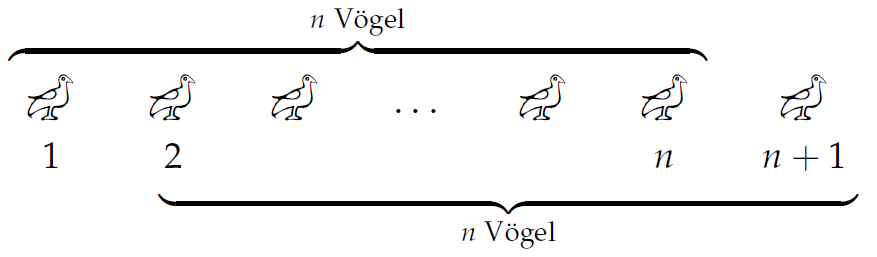
\includegraphics[scale=0.4]{induktion_voegel}
			\centering
		\end{figure}
	
		\only<5|handout:4>{
			Die Vögel $1, 2, ..., n$ bilden eine Menge mit genau $n$ Vögeln. Also haben sie nach Induktionsvoraussetzung alle die gleiche Farbe.\\ 
			Die Vögel $2, 3, ..., n + 1$ bilden auch eine Menge mit genau $n$ Vögeln. Also haben nach Induktionsvoraussetzung auch diese alle die gleiche Farbe.\\
			Folglich haben auch die Vögel $1$ und $n + 1$ die gleiche Farbe, also haben alle Vögel die gleiche Farbe.
		}
	\end{block}
	}
\end{frame}

\begin{frame}{Vogelfarben: Auflösung}
	\begin{figure}
		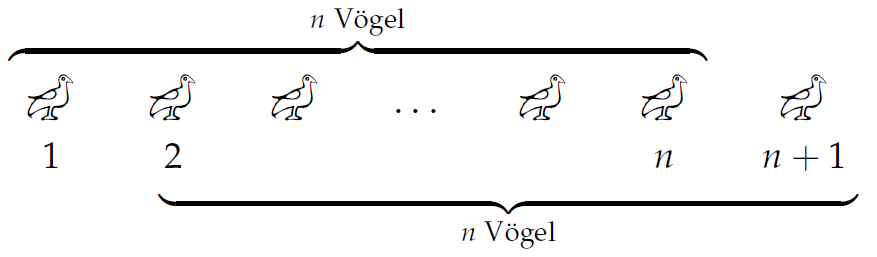
\includegraphics[scale=0.4]{induktion_voegel}
		\centering
	\end{figure}
	Das Bild ist zwar außerordentlich hübsch, suggeriert aber leider etwas, was nicht
	immer stimmt: Für $n = 2$ überlappen sich die Teilmengen „ohne den ersten“ und
	„ohne den letzten“ Vogel nicht. Es ist also nicht erzwungen, dass beide Vögel die
	gleiche Farbe haben.
	(Und das macht „alles weitere“ auch kaputt: Wenn nicht immer 2 Vögel die
	gleiche Farbe haben, dann auch nicht immer 3 Vögel, usw.)
\end{frame}

% Induktion Übung
% -------------------------
% Hier kommt noch was
% -------------------------

% Induktion Wörter Länge
\begin{frame}{Und jetzt mit Wörtern}
	\begin{block}{Behauptung}
		Seien $A, B$ zwei beliebige Alphabete. Definiere die Funktion $f: A^* \to A^*$
		\begin{align*}
			f(\eps) &= \eps \\
			\text{Für } w \in A^*, \mu \in A: f(\mu \· w) &= 
			\begin{cases}
				\mu \· f(w) &\mu \in B \\
				f(w) &\text{sonst}
			\end{cases}\\
		\end{align*}
	
	Dann gilt: $\forall w \in A^*: \size{f(w)} \le \size w$
	\end{block}
\end{frame}

\begin{frame}{Und jetzt mit Wörtern}
	Induktion über die Wortlänge ($n = \size w$):\\[0.5em]
	\begin{block}{Induktionsanfang}
		$n = 0$: Nur das leere Wort hat Länge 0. Also $w = \eps$\\
		$f(\eps) = \eps \impl \size{f(w)} = \size w = 0$
	\end{block}
	\begin{block}{Induktionsvoraussetzung}
		Für ein $n \in \N_0$ gelte: Für alle Wörter der Länge $n$ über $A$ (also $w \in A^n$) ist $\size{f(w)} \le \size w$
	\end{block}
\end{frame}

\begin{frame}{Und jetzt mit Wörtern}

	\begin{block}{Induktionsschluss}
		Zeige die Aussage für $n+1$:\\
		Sei $w \in A^{(n+1)}$ ein Wort der Länge $n+1$.\\
		Dann teilen wir es auf in $w = \mu \· v$ wobei $\mu \in A$ und $v \in A^n$.\\
		Nach IV gilt: $\size{f(v)} \le \size v$\\
		Fall 1: $\mu \in B$: $f(w) = \mu \· f(v)$ \impl $\size{f(w)} = 1 + \size{f(v)} \le 1 + \size v = 1+n = \size w$\\
		Fall 2: $\mu \notin B$: $f(w) = f(v)$ \impl $\size{f(w)} = \size{f(v)} \le \size v = n \le n+1 = \size w$\\
		\smallskip
		Also gilt: $\size{f(w)} \le \size w$
	\end{block}
\end{frame}

\section{Sprachen: Aufwärmen}


\begin{frame}{Rückblick}
	\begin{itemize}
		\item \textbf{Alphabet} $A$ mit Zeichen, aus denen wir Wörter zusammenbauen
		\item Nicht immer haben all diese Wörter einen Sinn
		\item Wir definieren selbst, welche Wörter wir als korrekt ansehen und akzeptieren wollen.
		\item Eine solche Teilmenge aller möglichen Wörter nennen wir \textbf{formale Sprache}
		%\item Das ist eine formale Sprache: Eine Teilmenge aller möglichen Wörter
	\end{itemize}
\end{frame}

\begin{frame}{Rückblick}
	Auf formale Sprachen können wir \textbf{ähnliche} Operationen anwenden wie auf Wörtern:
	\begin{itemize}
		\item $L_1 \cdot L_2 = \{w_1 w_2 \mid w_1 \in L_1 \text{ und } w_2 \in L_2 \}$\\
		Jeweils ein Wort aus $L_1$ konkateniert mit einem Wort aus $L_2$.
		\pause
		\item $L^0 = \{\varepsilon \}, \qquad L^{i+1} = L^i \cdot L$\\
		Alle Wörter, die aus $i = 0,1,2...$ Wörtern der Sprache zusammengesetzt wurden
		\pause
		\item $L^+ = \bigcup \limits_{i=1}^\infty L^i \qquad L^* = L^+ \cup L^0$\\
		Alle Wörter, die sich aus den Wörtern der Sprache bilden lassen \\ 
		(ohne/mit zusätzlichem $\eps$ als Würze).
	\end{itemize}
	Ein Alphabet selbst ist \textbf{auch} ne formale Sprache, nämlich mit Wörtern der Länge 1.
\end{frame}

\begin{frame}[t]{Wahr oder falsch?}
	\FalseQuestionE{Jede Sprache enthält Wörter.}{ $\emptyset$ ist auch eine gültige Sprache.}
	\FalseQuestionE{$\word{01}^* = \{\eps, \word{01}, \word{0101}, ...\}$}{$\word{01}^*$ gibt es nicht, denn $\word{01} \neq \{\word{01}\}$.}
	\TrueQuestionE{Es gibt Sprachen $L$, für die gilt $\eps \in L^+$.}{}
	\FalseQuestionE{$L^+ = L^* \setminus L^0$.}{Gilt nicht, wenn $\varepsilon \in L$.}
	\TrueQuestionE{$\{\}^* \neq \{\} $.}{ $\{\}^* = \{\varepsilon\}$.}	
\end{frame}

\def\mycircle{\raisebox{1pt}{\Circle}}

\morescalingdelimiters

\begin{frame}{Zum Aufwärmen: Sprache gesucht!} 
	Haben Alphabet $A = \{ \mword \triangle, \mword \square, \mword \mycircle \}$.\\
\end{frame}

%\begin{frame}
%	\frametitle{Zum Aufwärmen: Sprache gesucht!}
%	
%	Ihr erhaltet eine Karte mit einer Beschreibung einer formalen Sprache über dem Alphabet $\Sigma = \{ \triangle, \square, \circ \}$.\\
%	Ziel ist es, jeweils alle Beschreibungen von gleichen Sprachen zu sammeln.\\
%	Dazu überlegt ihr euch zunächst in 4er-Gruppen, ob ihr Beschreibungen von gleichen Sprachen habt oder was andere Beschreibungen wären. \\
%	Dann tauschen sich jeweils 3 4er-Gruppen aus und sammeln die Beschreibungen.
%\end{frame}

\begin{frame}{Zum Aufwärmen: Sprache gesucht!}
	
	Die Sprache der Wörter, die mit einem Kreis beginnen und danach keinen Kreis mehr enthalten.
	\bigskip
	\pause
	
	$$ \{\mword \mycircle\} \cdot \{\mword \triangle, \mword \square\}^* $$
	\bigskip
	\pause
	
	$$ \set{w \in A^* \mid w = \mword \Circle \cdot v, v \in \{\mword \triangle, \mword \square\}^* } $$

\end{frame}

\begin{frame}{Zum Aufwärmen: Sprache gesucht!}
	
	Die Sprache der Wörter, deren vorletztes Zeichen ein Dreieck ist.
	\bigskip
	\pause
	
	$$ \{\mword \triangle, \mword \square, \mword \mycircle\}^* \cdot \set{\mword \triangle} \cdot \{\mword \triangle, \mword \square, \mword \mycircle\} $$
	\bigskip
	\pause

	$$ \{w \in A^* \mid w = v \cdot \mword \triangle \cdot z, v \in A^*, z \in A \} $$

	
\end{frame}

\begin{frame}{Zum Aufwärmen: Sprache gesucht!}
	Die Sprache der Wörter, in denen nirgends eine ungerade Anzahl an Dreiecken nebeneinander steht.
	\bigskip
	\pause
	$$ \left(\{\mword \square, \mword \mycircle\}^* \cdot \{\mword \triangle\mword \triangle\}^* \right)^* $$
\end{frame}

\begin{frame}{Zum Aufwärmen: Sprache gesucht!}
	
	
	Die Sprache der Wörter, in denen eine gerade Anzahl an Vierecken vorkommt.
	\bigskip
	\pause
	$$ \{\mword \triangle, \mword \mycircle\}^* \cdot \left( \{\mword \square\} \cdot \{\mword \triangle, \mword \mycircle\}^* \cdot \{\mword \square\} \cdot \{\mword \triangle, \mword \mycircle\}^* \right)^* $$
	

\end{frame}

\begin{frame}{Zum Aufwärmen: Sprache gesucht!}
	Die Sprache der Wörter, in denen nirgends zwei Kreise aufeinander folgen.
	\bigskip
	\pause
	$$ \{\mword \square, \mword \triangle\}^* \cdot \left( \{\mword \mycircle\} \cdot \{\mword \square, \mword \triangle\}^+ \right)^* \cdot \{\mword \mycircle, \varepsilon\} $$
	

	
\end{frame}

\section{Formale Sprachen}

\begin{frame}
	\frametitle{Beispiel}
	Sei $A = \{a,b\}$ ein Alphabet. Mit $L$ wollen wir alle Wörter beschreiben, die genau ein $b$ enthalten. \\ \pause
	$$ L = \{w_1 b w_2 \mid w_1, w_2 \in \{a\}^\ast \}  \qquad  L = \{a\}^\ast \cdot \{b \} \cdot \{a\}^\ast$$
	
	Was ist $L^3$? Was enthält $L^i$? \pause
	Zum Beispiel ist $$aaababaaaabaa = aaaba \ baa \ aabaa \in L_3$$ \pause
	$L^i$ enthält alle Wörter, die genau $i$-mal ein $b$ enthalten! \\[1em]
	
	Was enthält $$L^i \setminus \{b\}^\ast$$ \pause
	Alle Wörter, die aus $i$ $b$'s bestehen, aber auch noch mindestens ein $a$ enthalten. \\
\end{frame}

\begin{frame}
	\frametitle{Aufgabe}
	Welche Eigenschaft muss eine formale Sprache $L$ über einem Alphabet
	$A$ erfüllen, damit gilt: $$ L^0 \subseteq L^1 \subseteq L^2 \subseteq L^3 \subseteq ... $$
	
	\pause
	\begin{block}{Lösung}
		Das gilt, wenn $$ \varepsilon \in L $$
	\end{block}
	
\end{frame}

\subsubsection{A1}
\begin{frame}
	\frametitle{Aufgabe (Klausur) \stars{4}}
		\begin{itemize}
			\item Wiederlegen Sie: Für alle formalen Sprachen $L_1 , L_2$ gilt: 
			$$L_1^\ast \cup L_2^\ast = (L_1 \cup L_2 )^\ast$$
			
			\item Zeigen Sie: Für alle formalen Sprachen $L$ gilt: 
				$$L^\ast \cdot L = L^+ $$ 
	\end{itemize}

	Tipp zu 2) (nicht in der Klausur gegeben): Hier handelt es sich um eine Mengengleichheit, also argumentieren wir mit \enquote{$\subseteq$} und \enquote{$\supseteq$}
\end{frame}

\begin{frame}
	\frametitle{Lösung}
	\textit{Für alle formalen Sprachen $L_1 , L_2$ gilt: 
		$$L_1^\ast \cup L_2^\ast = (L_1 \cup L_2 )^\ast$$ } \\[2em] \pause
	Diese Aussage ist falsch: Sei $L_1 = \{a\}$ und $L_2 = \{b\}$. Dann liegt \code{ab} in $(L_1 \cup L_2 )^\ast = \{a, b\}^\ast$ aber nicht in $L_1^\ast \cup L_2^\ast = \{a\}^\ast \cup \{b\}^\ast$.
\end{frame}

\begin{frame}
	\frametitle{Lösung}
	\textit{Für alle formalen Sprachen $L$ gilt: 
		$$L^\ast \cdot L = L^+ $$ } \\[1em] \pause
	Diese Aussage ist wahr! 
	\begin{block}{1. Schritt: $L^\ast \cdot L \subseteq L^+$:} \pause
	Wenn $w \in L^\ast \cdot L$ liegt, dann lässt es sich in Teilwörter auftrennen $$ w = w_1 \cdot w_2$$ mit $w_1 \in L^\ast$ und $w_2 \in L$. Für $w_1$ existiert ein $i \in \N_0$ mit $w_1 \in L^i$. Also $$w = w_1 w_2 \in L^i \cdot L = L^{i+1} \subset L^+$$
	\end{block}
\end{frame}

\begin{frame}
	\frametitle{Lösung}
	\textit{Für alle formalen Sprachen $L$ gilt: 
		$$L^\ast \cdot L = L^+ $$ } \\[1em] 
	Diese Aussage ist wahr! 
	\begin{block}{2. Schritt: $L^\ast \cdot L \supseteq L^+$:} \pause
	Wähle nun $w \in L^+$. Dann existiert ein $i \in \N_+$ mit $w \in L^i$. Da $i > 0$ lässt es sich schreiben als $i = j + 1$ für ein $j \in \N_0$. Also ist $$w \in L^{j+1} = L^j \cdot L \subset L^\ast \cdot L$$
	\end{block}
\end{frame}

\subsubsection{A2}
\begin{frame}
	\frametitle{Aufgabe (WS 2008) \stars{3}}
	Es sei $A = \{a, b\}$. Die Sprache $L \subset A^\ast$ sei definiert durch $$L = (\{a\}^\ast \cdot \{b\} \cdot \{a\}^\ast)^\ast$$
	Zeigen Sie, dass jedes Wort $w$ aus $\{a, b\}^\ast$, das mindestens einmal das Zeichen
	$b$ enthält, in $L$ liegt. (Hinweis: Führen Sie eine Induktion über die Anzahl der
	Vorkommen des Zeichens $b$ in $w$ durch.)
\end{frame}

\begin{frame}
	\frametitle{Lösung}
	$$L = (\{a\}^\ast \cdot \{b\} \cdot \{a\}^\ast)^\ast$$
	Sei $k$ die Anzahl der Vorkommen von $b$ in einem Wort $w \in \{a, b\}^\ast$.
	\begin{block}{Induktionsanfang}  \pause
		Für $k = 1$: In diesem Fall lässt sich das Wort $w$ aufteilen in $$w = w_1 \cdot b \cdot w_2$$ wobei $w_1$ und $w_2$ keine $b$ enthalten und somit in $\{a\}^\ast$ liegen. Damit gilt $w \in \{a\}^\ast \cdot \{b\} \cdot \{a\}^\ast$ und somit auch $$w \in (\{a\}^\ast \cdot \{b\} \cdot \{a\}^\ast)^\ast = L$$
	\end{block}
\end{frame}

\begin{frame}
	\frametitle{Lösung}
	\begin{block}{Induktionsannahme}  \pause
		Für ein festes $k \in \N$ gilt, dass alle Wörter über $\{a, b\}^\ast$, die genau $k$-mal das Zeichen $b$ enthalten, in $L$ liegen.
	\end{block} \pause
	\begin{block}{Induktionsschritt}  \pause
		Wir betrachten ein Wort $w$, das genau $k + 1$ mal das Zeichen $b$ enthält. Dann kann man $w$ zerlegen in $w$ = $w_1 \cdot w_2$, wobei $w_1$ genau einmal das Zeichen $b$ enthält und $w_2$ genau $k$-mal das Zeichen $b$. \pause Nach Induktionsanfang liegt $w_1$ in $\{a\}^\ast \{b\}\{a\}^\ast$. Nach Induktionsvoraussetzung liegt $w_2$ in $(\{a\}^\ast \{b\}\{a\}^\ast )^\ast$, was bedeutet, dass $w = w_1 \cdot w_2$ in $$(\{a\}^\ast \{b\}\{a\}^\ast )(\{a\}^\ast \{b\}\{a\}^\ast )^\ast \subseteq (\{a\}^\ast \{b\}\{a\}^\ast )^\ast = L$$ liegt und die Behauptung ist gezeigt.
	\end{block}
\end{frame}

%\subsubsection{A3}
%\begin{frame}
%	\frametitle{Noch mehr Aufgaben}
%	Begründen oder widerlegen Sie:
%	\begin{itemize}
%		\item Für alle formalen Sprachen $L$ gilt: 
%		$$(L_1^\ast \cdot L_2^\ast)^\ast = (L_1 \cdot L_2)^\ast$$ 
%		
%		\item Für alle formalen Sprachen $L_1 , L_2$ gilt: 
%		$$(L_1^\ast \cup L_2^\ast)^\ast = (L_1 \cup L_2 )^\ast$$
%	\end{itemize}
%\end{frame}
%
%\begin{frame}
%	\frametitle{Lösung}
%	\textit{Für alle formalen Sprachen $L_1 , L_2$ gilt: 
%		$$(L_1^\ast \cdot L_2^\ast )^\ast = (L_1 \cdot L_2 )^\ast$$ } \\[2em] \pause
%	Diese Aussage ist falsch: Sei $L_1 = \{a\}$ und $L_2 = \{b\}$. Dann liegt $$\mathbf{aa} = \mathbf{aa} \cdot \varepsilon$$ in $(L_1^\ast \cdot L_2^\ast ) = (L_1^\ast \cdot L_2^\ast )^1 \subset (L_1^\ast \cdot L_2^\ast )^\ast$, aber nicht in $(L_1 \cdot L_2 )^\ast = \{ab\}^\ast$.
%	
%\end{frame}
%
%\begin{frame}
%	\frametitle{Lösung}
%	\textit{Für alle formalen Sprachen $L_1 , L_2$ gilt: 
%		$$(L_1^\ast \cup L_2^\ast )^\ast = (L_1 \cup L_2 )^\ast$$ } \\[2em] \pause
%	Die Aussage ist korrekt: Sei $w$ ein Wort aus $(L_1^\ast \cup L_2^\ast )^\ast$. Dieses lässt sich in Teilwörter $w_1 , \cdots , w_k$ unterteilen, so dass für $1 \leq i \leq k$ gilt: 
%	$$w_i \in (L_1^\ast \cup L_2^\ast ) \implies w_i \in L_1^\ast \text{ oder } w_i \in L_2^\ast$$
%	Diese Teilwörter $w_i$ lassen sich wieder in Teilwörter $w_{i_1}, \dots w_{i_s}$ zerlegen, die entweder aus $L_1$ kommen, wenn $w_i \in L_1^\ast$ liegt, oder in $L_2$ liegen, wenn $w_i \in L_2^\ast$ liegt. Damit lässt sich $w$ in Teilwörter $w_{i_j}$ aus $L_1 \cup L_2$ unterteilen und es folgt $w \in (L_1 \cup L_2 )^\ast$. 
%\end{frame}
%
%\begin{frame}
%	\frametitle{Lösung}
%	\textit{Für alle formalen Sprachen $L_1 , L_2$ gilt: 
%		$$(L_1^\ast \cup L_2^\ast )^\ast = (L_1 \cup L_2 )^\ast$$ } \\[2em]
%	Sei umgekehrt ein Wort $w$ aus $(L_1 \cup L_2 )^\ast$. Dieses lässt sich dann in Teilwörter $w_1, \dots, w_k$ unterteilen, so dass für $1 \leq i \leq k$ gilt 
%	$$w_i \in L_1 \cup L_2 \implies w_i \in L_1 \subset L_1^\ast \text{ oder } w_i \in L_2 \subset L_2^\ast$$
%	Somit lässt sich $w$ in Teilwörter aus $L_1^\ast \cup L_2^\ast$ unterteilen, und es folgt $w \in (L_1^\ast \cup L_2^\ast )^\ast$.
%\end{frame}

\begin{frame}{Ausblick: Klammerausdrücke}
	
	Was ist mit der Sprache aller gültigen Klammerausdrücke? Können wir die auch mit $\set{}$, $\·$, ${}^*$ und ${}^+$ angeben? \only<beamer:0>{\\ \emph{Spoiler: Nein, das geht nicht!}}\\[1em]
	\pause
	
	\begin{block}{}
		\Large
		\centering
		COMING SOON... \\[1em]
	\end{block}

	\begin{figure}[H]
		\centering
		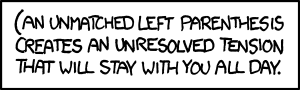
\includegraphics[scale=0.7]{xkcd/(.png}
		\vspace{-7pt}
		\caption{ \texttt{\url{https://xkcd.com/859/}} }
	\end{figure}
\end{frame}

%\section{Von der Darstellung zur Zahl}

\subsection{Definitionen}
\begin{frame}{Numerischer Wert einer Ziffernfolge}
	\begin{Definition}
		Zu einer Zahlenbasis $b$ definiere 
		\begin{align*}
			\fnum_b &\from Z_b \functionto \Z \\
			\fnum_b(x) &:= x \text{ (als Zahl)} \quad \text{für einzelne Ziffern $x \in Z_b$} \\
			& \\
			\fNum_b &\from Z_b^* \functionto \Z \\
			\fNum_b(\eps) &:= 0 \\
			\fNum_b(wx) &:= b\cdot \fNum_b(w) + \fnum_b(x) \quad \text{ für alle } w\in Z_b^\ast, x\in Z_b. 
		\end{align*}
	\end{Definition}

	\pause
	\textbf{Hinweis}: $\fNum_b$ ist eine Abbildung, die einem Wort (Zahlendarstellung) eine Zahl (Wert) zuordnet. \\
	Wir schreiben für die Zahl aber wieder eine Darstellung hin (nämlich im Dezimalsystem).
\end{frame}
\begin{frame}{Aufgabe}
	Berechnet die Zahlenwerte von $ \word{11}_2, \word{321}_4, \word{B2}_{16}$.
	\begin{align*} 
	\fNum_2(\word{11}) &= \visible<2->{2\cdot \fNum_2(\word 1) + \fnum_2(\word 1) \\
	&= 2\cdot 1 + 1 \\
	&= 3  \\}
	\visible<3->{\fNum_4(\word{321}) &=} \visible<4->{ 4\cdot \fNum_4(\word{32}) + \fnum_4(\word 1) \\
	&= 4\cdot \left( 4\cdot \fNum_4(\word 3) + \fnum_4(\word 2) \right) + \fnum_4(\word 1) \\
	&= 4^2\cdot \fnum_4(\word 3) + 4 \cdot \fnum_4(\word 2) + \fnum_4(\word 1) \\
	&= 57 \\}
	\visible<5->{\fNum_{16}(\word{B2}) &=} \visible<6->{ 16 \cdot \fNum_{16}(\word B) + \fnum_{16}(\word 2) \\
	&= 16\cdot 11 + 2 \\
	&= 178}
	\end{align*}

\end{frame}

\mycomment{  % man sieht hier nicht viel...
	\begin{frame}{Wohldefiniertheit}
		\emph{Behauptung}: Die Definition 
			$$ \fNum_b(\eps) = 0  $$  
			$$ \fNum_b(wx) = b\cdot \fNum_b(w) + \fnum_b(x) \text{ für alle } w\in Z_b^\ast, x\in Z_b $$ 
			ist wohldefiniert und weist jedem Wort eine eindeutige Bedeutung zu, die dem Zahlenwert entspricht.
	\end{frame}
	\begin{frame}{Beweis}
		\begin{block}{Beweis durch vollständige Induktion über $n=\vert w \vert $}
		\begin{itemize}
			\only<1-2>{\item<1->[{IA.:}] $n = 0 = \vert w \vert \implies w = \eps $. \\
			Für $w = \eps $ ist $\fNum_b$ wohldefiniert und sinnvoll (nämlich $\fNum_b(\eps) = 0$).
			\item<2->[{IV.:}] Für ein beliebig aber festes $n\in\N_0$ sei $\fNum_b(w)$ für alle $w$ mit $\setsize{w} = n$ wohldefiniert und entspreche dem Zahlenwert. }
			\only<3->{\item<3->[{IS.:}] Wähle $w'$ mit $\vert w' \vert = n+1 $, dann gibt es ein $w\in Z_b^n, x\in Z_b$, so dass $ w' = wx $ \\
			Mit der Definition gilt nun $$ \fNum_b(w') = b\cdot {\underbrace{\fNum_b(w)}_{IV}} + \fnum_b(x) $$
			Die Summe ist laut $IV$ wohldefiniert. Auch ist laut $IV$ $\fNum_b(w)$ der Zahlenwert von $w$ und damit auch $\fNum_b(w')$.}
		\end{itemize}
		\end{block}
	
	\end{frame}
}

%\subsection{Aufgabe}
%\begin{frame}{Aufgabe. WS 2010 }
%Es bezeichne $\Z$ die Menge der ganzen Zahlen. Gegeben sei eine Ziffernmenge $Z_{-2} = \{N, E\}$ mit der Festlegung $num_2 (N) = 0$ und $num_2 (E) = 1$. Wir definieren eine Abbildung $\fNum_{-2} : Z_{-2}^\ast \functionto \Z$ wie folgt:
%	$$\fNum_{-2} (\eps) = 0$$
%	$$\forall \ w \in Z_{-2}^\ast \ \forall \ x \in Z_{-2} : \fNum_{-2} (wx) = -2 \cdot \fNum_{-2} (w) + num_2 ( x )$$
%
%	\begin{itemize}	
%		\item Geben Sie für $w \in \{E, EN, EE, ENE, EEN, EEE\}$ jeweils $\fNum_{-2} (w)$ an.
%		\item Für welche Zahlen $x \in \Z$ gibt es ein $w \in Z_{-2}^\ast$ mit $\fNum_{-2} (w) = x$?
%	\end{itemize}
%\end{frame}
%
%\begin{frame}{Lösung}
%\textit{Geben Sie für $w \in \{E, EN, EE, ENE, EEN, EEE\}$ jeweils $\fNum_{-2} (w)$ an.} \pause
%	\begin{table}[h!]	
%		\begin{tabular}{>{$}l<{$}>{$}l<{$}}
%			\fNum_{-2} (E)\pause & = 1 \\ \pause 
%			\fNum_{-2} (EN)\pause & = -2 \\ \pause
%			\fNum_{-2} (EE)\pause & = -1 \\ \pause
%			\fNum_{-2} (ENE)\pause & = 5 \\ \pause
%			\fNum_{-2} (EEN)\pause & = 2 \\ \pause
%			\fNum_{-2} (EEE)\pause & = 3
%	\end{tabular}
%	\end{table}
%	\pause
%	\textit{Für welche Zahlen $x \in \Z$ gibt es ein $w \in Z_{-2}^\ast$ mit $\fNum_{-2} (w) = x$?} \\[1em]\pause
%	Für alle!
%\end{frame}

\section{Von der Zahl zur Darstellung}
\begin{frame}{Division und Modulo}
	\begin{block}{Definition}
		$ x \div y$ ist die ganzzahlige Division von x durch y.\\
		$ x \mod y$ liefert den Rest dieser Division.
	\end{block} 
	\pause
	
	\begin{block}{Beobachtung}
		$ x\div y \in \N_0, \qquad x\mod y \in \{0,\dots, y-1\} $
	\end{block}
	\pause
	
	\begin{Beispiel}
		\begin{tabular}{c|cccc|cccc}
			$y$ & \multicolumn{4}{c|}{2} & \multicolumn{4}{c}{3} \\
			$x$ & 1 & 2 & 5 & 8 & 1 & 2 & 5 & 8 \\ \pause
			$x\div y$ & 0 & 1 & 2 & 4 & 0 & 0 & 1 & 2 \\
			$x\mod y$ & 1 & 0 & 1 & 0 & 1 & 2 & 2 & 2 \\
		\end{tabular}
	\end{Beispiel}
	
\end{frame}

\begin{frame}{Division und Modulo}

	\begin{block}{Lemma}
		$$ x = y \cdot (x \div y ) + \left( x \mod y \right)$$ 
	\end{block}

	\begin{Beispiel}
		\begin{table}[h!]
			\centering
			\begin{tabular}{c|cccccccccccc}
				$x$ & 0 & 1 & 2 & 3 & 4 & 5 & 6 & 7 & 8 & 9 & 10 & 11 \\ \hline
				$x\div 4 $ & \only<2->{0 & 0 & 0 & 0 & 1 & 1 & 1 & 1 & 2 & 2 & 2 & 2 } \only<1|handout:0>{&&&&&&&&&&&} \\
				$x\mod 4$ & \only<3->{0&1&2&3&0&1&2&3&0&1&2&3} \only<1-2|handout:0>{&} \\
				$4 \· \left( x\div 4\right) $ & \only<4->{0&0&0&0&4&4&4&4&8&8&8&8} \only<1-3|handout:0>{&&&&&&&&&&}  \\ \hline
				$4 \· \left( x\div 4\right) + x \mod 4 $ & \only<5->{0 & 1 & 2 & 3 & 4 & 5 & 6 & 7 & 8 & 9 & 10 & 11} \only<1-4|handout:0>{&&&&&&&&&&}
			\end{tabular}
		\end{table}
	\end{Beispiel}

	\visible<5-> {$ \Impl$ \enquote{Beweis durch Beispiel} :P \qed}

\end{frame}

\begin{frame}{Repräsentation von Zahlen}
	Wir definieren
	\begin{threealign}
	\fRepr_k \from \; \N_0 &\functionto& Z_k,  \\
	n &\mapsto& \begin{cases} \frepr_k(n), & n<k \\ \fRepr_k\left( n\div k \right) \cdot \frepr_k\left( n \mod k \right), & n\geq k 
	\end{cases}.
	\end{threealign}
	\pause
	\begin{block}{Es gilt}
		$\fRepr_k(n)$ ist das kürzeste Wort $w\in Z_k^\ast$ mit $\fNum_k(w)=n$, also 
		$$ \fNum_k\left( \fRepr_k(n)\right) = n. $$ 
	\end{block}
	\pause
	\emph{Anmerkung}:
	Im Allgemeinen ist $$ \fRepr_k\left(\fNum_k(w)\right) \neq w, $$ da überflüssige Nullen in $w$ wegfallen können. 
\end{frame}

\begin{frame}{Repräsentation von Zahlen}
	\begin{threealign}
	\fRepr_k : \; \N_0 &\functionto& Z_k,  \\
	n &\mapsto& \begin{cases} \frepr_k(n), & n<k \\ \fRepr_k\left( n\div k \right) \cdot \frepr_k\left( n \mod k \right), & n\geq k 
	\end{cases}
	\end{threealign}
	
	\begin{block}{Aufgabe}
		Berechnet folgende Darstellungen:\\
		$\fRepr_2(42) = \only<2->{\word{101010}}$ \\
		$\fRepr_4(42) = \only<3->{\word{222}}$ \\
		$\fRepr_8(42) = \only<4->{\word{52}}$ \\
		$\fRepr_{16}(42) = \only<5->{\word{2A}}$
	\end{block}
\end{frame}

\begin{frame}{Beispiel: ausführl. Lösung}
	\begin{align*}
		\fRepr_8(42) &= \fRepr_8(42 \div 8) \cdot \frepr_8(42 \mod 8) \\
		&= \fRepr_8(5) \cdot \frepr_8(2)\\
		&= \frepr_8(5) \cdot \word 2\\
		&= \word 5 \cdot \word 2\\
		&= \word{52}_8\thassedaniel{}{.}
	\end{align*}
	
\end{frame}


\begin{frame}	
	\begin{block}{Was ihr nun wissen solltet}
		\begin{itemize}
			\item Wie man wahre Aussagen konstruiert \qquad (\#NoFakeNews!) 
			\item Wie vollständige Induktion geht
			\item Wie man formale Sprachen angeben kann
			\item Wie man Beweise mit formalen Sprachen führt
		\end{itemize}
	\end{block}
	
	\begin{block}{Was nächstes Mal kommt}
		\begin{itemize}
			\item Wie man von Zahlendarstellungen zu Zahlen kommt...
			\item[] ... und wieder zurück
			\item Nicht immer so positiv: Negative Zahlen
			%\item Komprimierung: Huffmann-Codierungen
		\end{itemize}
	\end{block}
\end{frame}

%% Letzte Seite
\thassedaniel{
	\lastframe{0.7}{0}{xkcd/1_to_10.png}{https://xkcd.com/953/} %TODO
}{
	\lastframetitled{0.7}{0}{xkcd/win_by_induction.png}{ https://xkcd.com/1516/}{Win by Induction}
}


\slideThanks

\end{document}
